%%%%%%%%%%%%%%%%%%%%%%%%%%%%%%%%%%%%%
%                                   %
% Compile with XeLaTeX and biber    %
%                                   %
% Questions or comments:            %
%                                   %
% joshua dot mcneill at uga dot edu %
%                                   %
%%%%%%%%%%%%%%%%%%%%%%%%%%%%%%%%%%%%%

\documentclass{beamer}
  % Read in standard preamble (cosmetic stuff)
  %%%%%%%%%%%%%%%%%%%%%%%%%%%%%%%%%%%%%%%%%%%%%%%%%%%%%%%%%%%%%%%%
% This is a standard preamble used in for all slide documents. %
% It basically contains cosmetic settings.                     %
%                                                              %
% Joshua McNeill                                               %
% joshua dot mcneill at uga dot edu                            %
%%%%%%%%%%%%%%%%%%%%%%%%%%%%%%%%%%%%%%%%%%%%%%%%%%%%%%%%%%%%%%%%

% Beamer settings
% \usetheme{Berkeley}
\usetheme{CambridgeUS}
% \usecolortheme{dove}
% \usecolortheme{rose}
\usecolortheme{seagull}
\usefonttheme{professionalfonts}
\usefonttheme{serif}
\setbeamertemplate{bibliography item}{}

% Packages and settings
\usepackage{fontspec}
  \setmainfont{Charis SIL}
\usepackage{hyperref}
  \hypersetup{colorlinks=true,
              allcolors=blue}
\usepackage{graphicx}
  \graphicspath{{../../figures/}}
\usepackage[normalem]{ulem}
\usepackage{enumerate}

% Document information
\author{M. McNeill}
\title[FREN2001]{Français 2001}
\institute{\url{joshua.mcneill@uga.edu}}
\date{}

%% Custom commands
% Lexical items
\newcommand{\lexi}[1]{\textit{#1}}
% Gloss
\newcommand{\gloss}[1]{`#1'}
\newcommand{\tinygloss}[1]{{\tiny`#1'}}
% Orthographic representations
\newcommand{\orth}[1]{$\langle$#1$\rangle$}
% Utterances (pragmatics)
\newcommand{\uttr}[1]{`#1'}
% Sentences (pragmatics)
\newcommand{\sent}[1]{\textit{#1}}
% Base dir for definitions
\newcommand{\defs}{../definitions}


  % Packages and settings

  % Document information
  \subtitle[Adjectifs prénominaux]{Les adjectifs prénominaux}

\begin{document}
  % Read in the standard intro slides (title page and table of contents)
  \begin{frame}
    \titlepage
    \tiny{Office: % Basically a variable for office hours location
Gilbert 121\\
          Office hours: % Basically a variable for office hours
 lundi, mercredi, vendredi 10:10--11:10
}
  \end{frame}

  \begin{frame}{Annonces}
    \begin{itemize}
      \item Les examens sont notés, mais je vais vous rendre plus tard. Vous pouvez trouvez vos notes sur eLC.
      \item[] \tinygloss{The exams are graded, but they'll be returned to you later. You can find your grades on eLC.}
    \end{itemize}
  \end{frame}

  \begin{frame}{Les adjectifs BRAGS}
    \begin{columns}
      \column{0.5\textwidth}
        C'est...
        \begin{enumerate}
          \item un \underline{\uncover<2->{vieux}} café \underline{\hspace{1cm}}
          \item<3-> un \underline{\uncover<4->{mauvais}} homme \underline{\hspace{1cm}}
          \item<5-> une \underline{\hspace{1cm}} femme \underline{\uncover<6->{intelligente}}
          \item<7-> une \underline{\uncover<8->{bonne}} carte \underline{\hspace{1cm}}
          \item<9-> un \underline{\hspace{1cm}} homme \underline{\uncover<10->{sportif}}
          \item<11-> un \underline{\uncover<12->{nouvel}} hôtel \underline{\hspace{1cm}}
        \end{enumerate}
      \column{0.5\textwidth}
        \begin{minipage}[c][0.6\textheight]{\linewidth}
          \begin{center}
            \only<1-2>{
              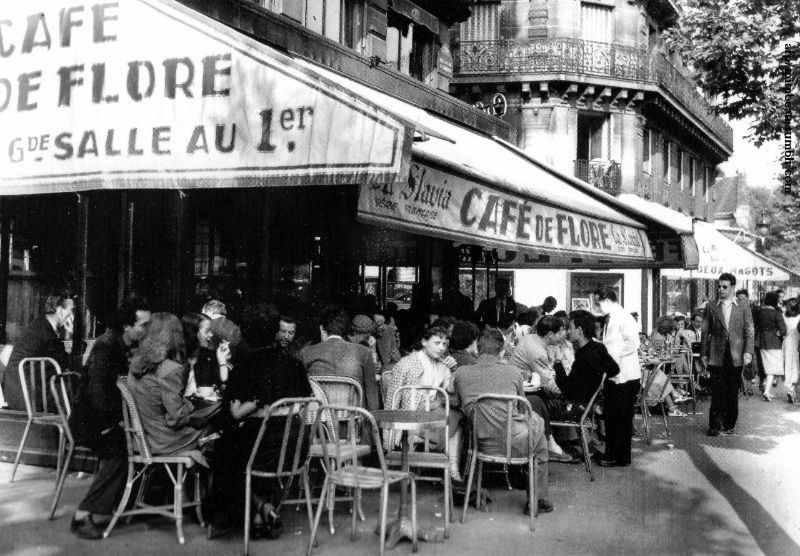
\includegraphics[scale=0.2]{cafe.jpg} \\
              Café de Flore à Paris \\
              \emph{Fondé en 1887}
            }
            \only<3-4>{
              
\includegraphics[scale=0.125]{thanos.jpg}
            }
            \only<5-6>{
              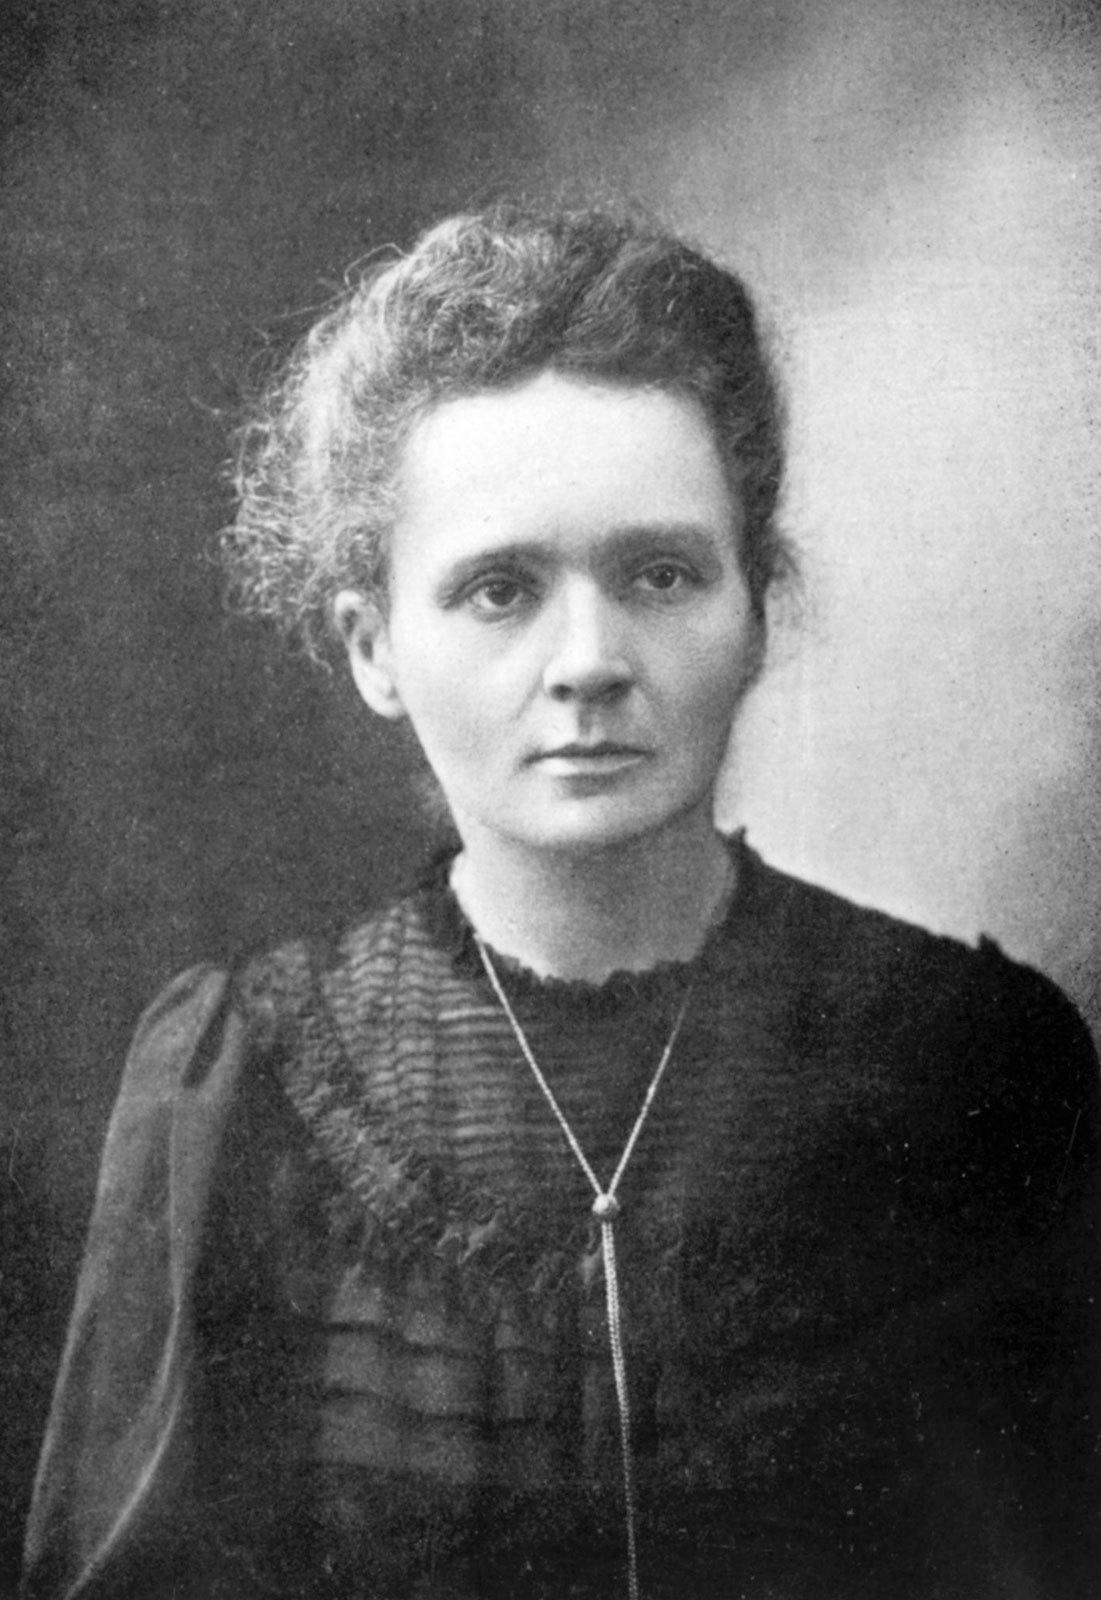
\includegraphics[scale=0.1]{marie_curie.jpg} \\
              Marie Curie
            }
            \only<7-8>{
              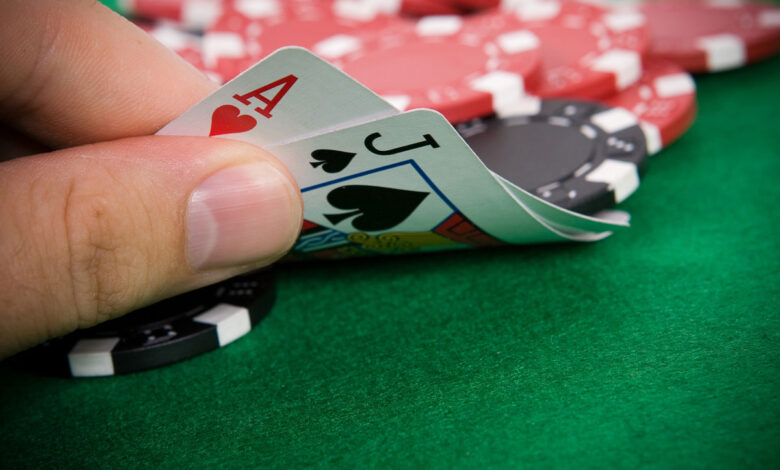
\includegraphics[scale=0.2]{blackjack.jpg}
            }
            \only<9-10>{
              
\includegraphics[scale=0.125]{lebron.jpg}
            }
            \only<11-12>{
              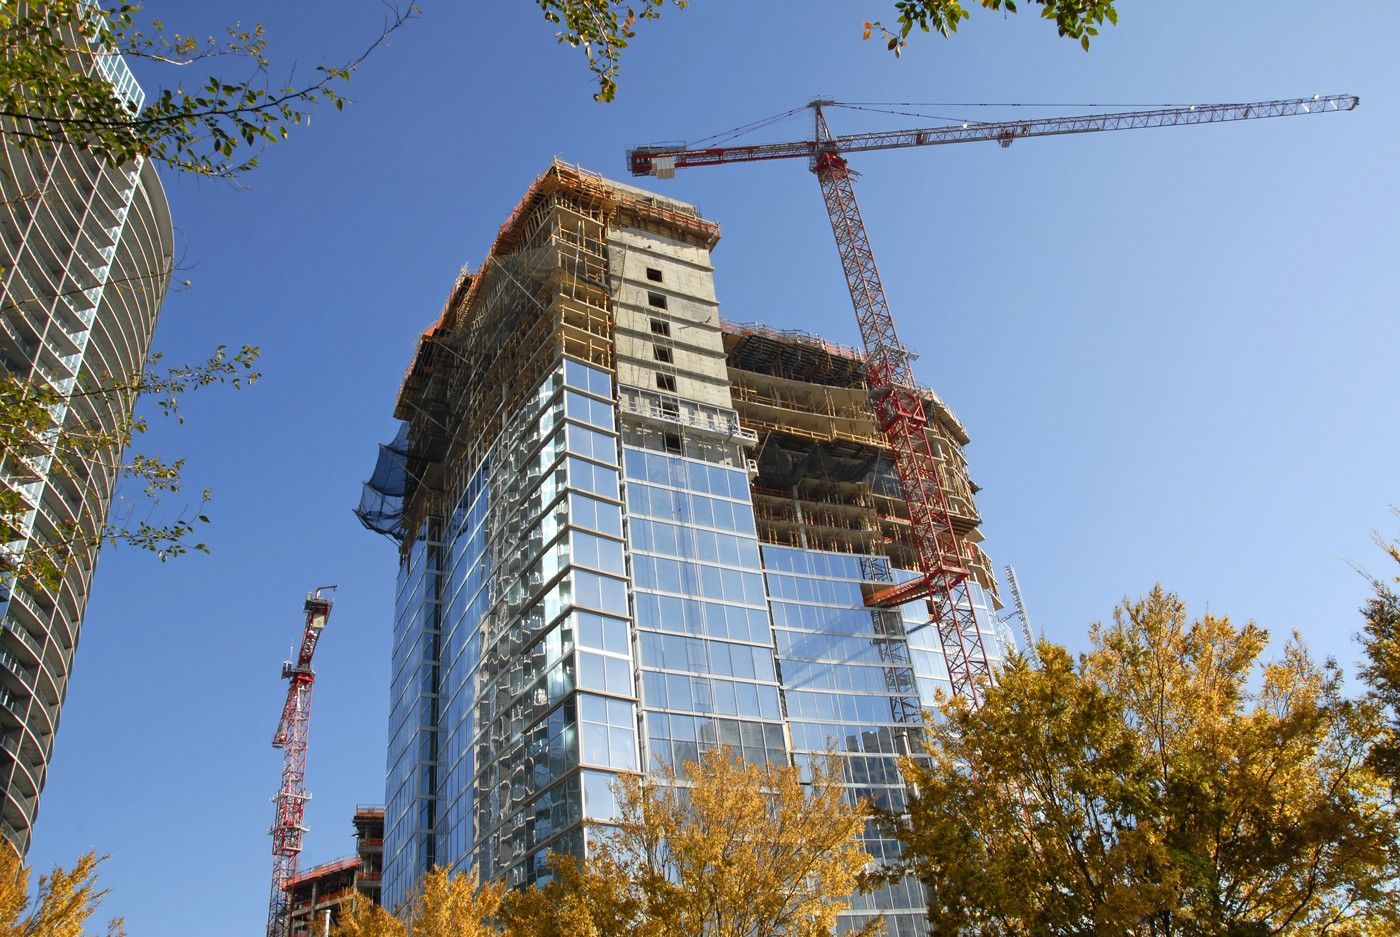
\includegraphics[scale=0.125]{hotel.jpg}
            }
          \end{center}
        \end{minipage}
    \end{columns}
  \end{frame}

  \begin{frame}{}
    \begin{center}
      \Large Quiz
    \end{center}
  \end{frame}

  \begin{frame}{Trouvez une personne...}
    \begin{columns}
      \column{0.5\textwidth}
        Pour chaque description, trouve un/e camarade de classe pour qui elle est vraie, puis écris le nom de ce/tte camarade. \\
        \tinygloss{For each description, find a classmate for whom it is true, then write down that classmate's name.}
      \column{0.5\textwidth}
        {\scriptsize
        \begin{description}
          \item[] \textbf{Modèle:}
          \item[] \emph{... qui a un bon prof de maths.}
          \item[E1:] Est-ce que tu as un bon prof de maths?
          \item[E2:] Non, je n'ai pas un bon prof de maths. (\emph{ask another classmate})
          \item[E3:] Oui, j'ai un bon prof de maths.
        \end{description}
        }
    \end{columns}
    \vspace{1cm}
    {\scriptsize
    \begin{columns}[t]
      \column{0.5\textwidth}
        \begin{enumerate}
          \item ... qui habite une vieille résidence.
          \item ... qui habite un bel appartement.
          \item ... qui a un nouvel ordinateur.
          \item ... qui a une petite voiture.
          \item ... qui a son premier cours à huit heures du matin.
        \end{enumerate}
      \column{0.5\textwidth}
        \begin{enumerate}
          \setcounter{enumi}{5}
          \item ... qui prépare un grand examen.
          \item ... qui est en première année de fac.
          \item ... qui est en dernière année de fac.
          \item ... qui a un bon prof de maths.
          \item ... qui a un vieil ami sur le campus.
        \end{enumerate}
    \end{columns}
    }
  \end{frame}

  \begin{frame}{Au contraire}
    Avec un partenaire, posez les questions suivantes chacun à ton tour.
    Fais répondre avec l'adjectif opposé à ton/ta partenaire. \\
    \tinygloss{With a partner, take turns asking the following questions.
    Have your partner respond with the opposite adjective.}
    \begin{center}
      \begin{description}
        \item[] \textbf{Modèle:}
        \item[E1:] C'est un vieux professeur?
        \item[E2:] Mais non, c'est un jeune professeur!
      \end{description}
      \begin{columns}
        \column{0.5\textwidth}
          \begin{enumerate}
            \item C'est un mauvais livre?
            \item C'est un vieil ordinateur?
            \item C'est le premier examen?
            \item C'est une grande piscine?
          \end{enumerate}
        \column{0.5\textwidth}
          \begin{enumerate}
            \setcounter{enumi}{4}
            \item C'est la dernière résidence?
            \item C'est un petit appartement?
            \item C'est un mauvais professeur?
            \item C'est un nouvel amphithéâtre?
          \end{enumerate}
      \end{columns}
    \end{center}
  \end{frame}

  \begin{frame}{}
    \begin{center}
      \Large Questions?
    \end{center}
  \end{frame}
\end{document}
